\documentclass[10pt]{mypackage}

% sans serif font:
%\usepackage{cmbright}
%\usepackage{sfmath}
%\usepackage{bbold} %better blackboard bold

%serif font + different blackboard bold for serif font
\usepackage{newpxtext,eulerpx}
\renewcommand*{\mathbb}[1]{\varmathbb{#1}}

\fancyhf{}
\rhead{Avinash Iyer}
\lhead{Mathematical Methods of Physics: Class Notes}

\setcounter{secnumdepth}{0}

\begin{document}
\section{Things You Just Gotta Know}%
\subsection{Coordinate Systems}%
We want to focus on vector-valued functions of coordinates.
\begin{align*}
  \vec{V}(\mathbf{r}) &= V_x(x,y)\hat{i} + V_y(x,y)\hat{j}.
\end{align*}
Notice that a vector function uses the coordinate system twice. Once for the function's inputs, once for the vectors themselves.
\subsubsection{Polar Coordinates}%
\begin{center}
  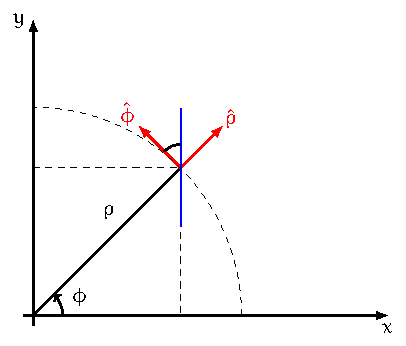
\includegraphics[width=10cm]{polar_coordinates.pdf}
\end{center}
We can also express the inputs to $ \vec{V} $ in polar coordinates, $(\rho,\phi)$.
\begin{align*}
  \vec{V}(\mathbf{r}) &= V_{\rho}\left(\rho,\phi\right)\hat{i} + V_{\phi}\left(\rho,\phi\right)\hat{j}.
\end{align*}
To extract the input functions, we take
\begin{align*}
  V_x &= \hat{i}\cdot \vec{V}\\
  V_y &= \hat{j}\cdot \vec{V}.
\end{align*}
Alternatively, we can project $ \vec{V} $ onto the $\hat\rho,\hat\phi$ axis:
\begin{align*}
  \vec{V}(\mathbf{r}) &= V_{\rho}\left(\rho,\phi\right)\hat{\rho} + V_{\phi}\left(\rho,\phi\right)\hat{\phi},
\end{align*}
and we extract
\begin{align*}
  V_{\rho} &= \hat{\rho}\cdot \vec{V}\\
  V_{\phi} &= \hat{\phi}\cdot \vec{V}.
\end{align*}
Notice that $\mathbf{r}$ is an abstract vector; we need to project it onto a basis.\newline

For instance, we can take the position vector and project it onto the cartesian and polar axes:
\begin{align*}
  \mathbf{s} &= x\hat{i} + y\hat{j}\\
             &= \rho \cos \phi \hat{i} + \rho \sin \phi \hat{j}\\
             &= \rho \hat{\rho}\\
             &= \sqrt{x^2 + y^2}\hat{\rho}
\end{align*}
The main reason we avoided using the $\hat\rho,\hat\phi$ axis up until this point is that $\rho$ and $\phi$ are \textit{position-dependent}, while the $\hat{i},\hat{j}$ axis is position-independent.\newline

Now, we must figure out the position-dependence of $\hat{\rho}$ and $\hat{\phi}$:
\begin{align*}
  d\mathbf{r} &= \pd{\mathbf{r}}{\rho}d\rho + \pd{\mathbf{r}}{\phi}d\phi.
\end{align*}
If we hold $\phi$ constant, it must be the case that any change in $\rho$ is in the $\hat\rho$ direction. Therefore,
\begin{align*}
  \hat\rho &= \frac{\pd{\mathbf{r}}{\rho}}{\left\Vert \pd{\mathbf{r}}{\rho} \right\Vert}\\
           &= \frac{\cos\phi\hat{i} + \sin\phi\hat{j}}{\left\vert \cos\phi\hat{i} + \sin\phi\hat{j} \right\vert}\\
           &= \cos\phi\hat{i} + \sin\phi\hat{j}.
\end{align*}
Similarly,
\begin{align*}
  \hat\phi &= \frac{\pd{\mathbf{r}}{\phi}}{\norm{\pd{\mathbf{r}}{\rho}}}\\
           &= \frac{-\rho\sin\phi\hat{i} + \rho\cos\phi\hat{j}}{\left\Vert -\rho\sin\phi\hat{i} + \rho\cos\phi\hat{j} \right\Vert}\\
           &= -\sin\phi\hat{i} + \cos\phi\hat{j}.
\end{align*}
Thus, we can see that the $\hat\rho,\hat,\phi$ axis is orthogonal. 
\begin{align*}
  \pd{\hat{\rho}}{\phi} &= -\sin\phi\hat{i} + \cos\phi\hat{j}\\
                        &= \hat{\phi},\\
  \pd{\hat{\phi}}{\phi} &= -\hat{\rho},\\
  \pd{\hat{\phi}}{\rho} &= 0,
  \intertext{and}
  \pd{\hat{\rho}}{\rho} &= 0
\end{align*}
\begin{example}[Velocity]
  \begin{align*}
    \mathbf{v} &= \frac{d \mathbf{s}}{dt}\\
               &= \frac{d}{dt}\left(x\hat{i}\right) + \frac{d}{dt}\left(y\hat{j}\right).
               \intertext{In the case of cartesian coordinates, $\hat{i}$ and $\hat{j}$ are constants.}
               &= v_{x}\hat{i} + v_{y}\hat{j}
  \end{align*}
  When we examine polar coordinates, since $\hat{\rho}$ and $\hat{\phi}$ are position-dependent, we must use the chain rule.\footnote{Note that $\hat{\rho} = \hat{\rho}\left(\rho,\phi\right)$ and $\hat{\phi} = \hat{\phi}(\rho,\phi)$.}
  \begin{align*}
    \mathbf{v} &= \frac{d\mathbf{s}}{dt}\\
               &= \frac{d\rho}{dt}\hat{\rho} + \rho \frac{d\hat{\rho}}{dt}\\
               &= \frac{d\rho}{dt}\hat{\rho} + \rho \left(\cancelto{0}{\pd{\hat{\rho}}{\rho}}\frac{d\rho}{dt} + \underbrace{\pd{\hat{\rho}}{\phi}}_{=\hat{\phi}}\frac{d\phi}{dt}\right)\\
               &= \frac{d\rho}{dt}\hat{\rho} + \rho \frac{d\phi}{dt}\hat{\phi}\\
               &= \dot\rho\hat\rho + \rho\dot\phi\hat\phi.
  \end{align*}
  Notice that $\dot\rho$ is the radial velocity and $\dot\phi = \omega$ is the angular velocity.
\end{example}
\subsubsection{Spherical Coordinates}%
\begin{center}
  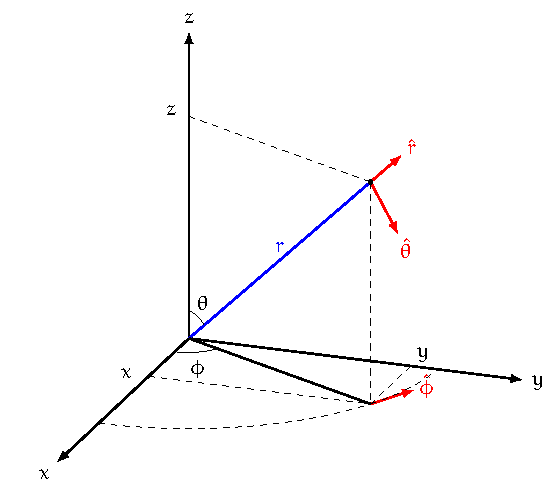
\includegraphics[width=10cm]{spherical_coordinates.pdf}
\end{center}
\begin{center}
  \renewcommand{\arraystretch}{1.5}
  \begin{tabular}{c|c|c}
    Polar & Cylindrical & Spherical\\
    \hline
    $\mathbf{s} = s(\rho,\phi)$ & $\mathbf{s} = s(\rho,\phi,z)$ & $\mathbf{s} = s(r,\phi,\theta)$\\
    $\mathbf{s} = \begin{pmatrix}\rho\cos\phi\\\rho\sin\phi\end{pmatrix}$ & $\mathbf{s} = \begin{pmatrix}\rho\cos\phi\\\rho\sin\phi\\z\end{pmatrix}$ & $\mathbf{s} = \begin{pmatrix}r\cos\phi\sin\theta\\r\sin\phi\sin\theta \\ r\cos\theta\end{pmatrix}$
  \end{tabular}
\end{center}
Here,\footnote{Physicists amirite?} $\phi$ denotes the polar angle and $\theta$ denotes the azimuthal angle. Notice that $\phi \in [0,2\pi)$ and $\theta \in [0,\pi]$.\newline

We can see that $\hat\rho$, $\hat\phi$, and $\hat\theta$ in spherical coordinates are also position-dependent.
\begin{align*}
  \hat r &= \frac{\pd{\mathbf{s}}{r}}{\norm{\pd{\mathbf{s}}{r}}}\\
         &= \sin\theta\cos\phi\hat{i} + \sin\theta\sin\phi\hat{j} + \cos\theta\hat{k}\\
  \hat{\phi} &= \frac{\pd{\mathbf{s}}{\phi}}{\norm{\pd{\mathbf{s}}{\phi}}}\\
             &= -\sin\phi\hat{i} + \cos\phi\hat{j}\\
  \hat{\theta} &= \frac{\pd{\mathbf{s}}{\theta}}{\norm{\pd{\mathbf{s}}{\theta}}}\\
               &= \cos\phi\cos\theta\hat{i} + \cos\theta\sin\phi\hat{j} - \sin\theta\hat{k}
\end{align*}
\end{document}
